\chapter{Mirror Descent} 
Gradient descent algorithm works well for smooth convex optimization problems. However, it's not the best
for specific classes of fucntions and bodies: for instance, for minimizing linear functions over the probablity
simplex. The general gradient descent algorithm does significantly worse than thte specialized Hedge algorithm.

Another example is about the curse of dimension. In high dimensions, the dimension-free oracle complexity is possible when the objective function $f$ and the constrained set $\cX$ are well-behaved in the Euclidean norm. However, if this assumption is not met, then the gradient descent techniques may lose their dimension-free convergence rates. For instance, if we consider a differnetiable convex function $f$ defined on the Euclidean ball s.t. $\|\nabla f(x)\|_\infty \le 1, \forall x \in B_{2,n}$. This implies $\|\nabla f(x) \|_2\le \sqrt{n}$ and thus the projected gradient descent will converge to the minimum of $f$ on $B_{2,n}$ at a rate of $\sqrt{\frac{n}{t}}$. Known as mirror descent,  the rate could be improved to $\sqrt{\frac{\log n}{t}}$.    

This suggests asking: {\it can we somehow change gradient descent to adapt to the ``geometry'' of the problem?}
This is the question that the Mirror Descent algorithm answers.

\section{Mirror Descent: the Proximal Point View} 
We know the proximal gradient descent algorithm.

\begin{algorithm}[H]
    \caption{Proximal Gradient Descent Algorithm}
    \label{algo PGD}
    $x_1$ starting point \; 
    \For{$t=1,2,\ldots,T$}{
        $x_{t+1} = \argmin_x \eta \langle \nabla f_t(x_t), x \rangle + \frac{1}{2}\|x-x_t\|^2 $\;
    }
\end{algorithm}

If we take the derivative, we can get the update rule:
$$
\eta \nabla f_t\left(x_{t}\right)+x_{t+1}-x_t=0 \Longrightarrow x_{t+1}=x_t-\eta \nabla f_t\left(x_{t}\right),
$$
which matches the normal gradient descent algorithm. The intuition also makes sense: if we want to minimize the function $f_t$, we could try to minimize its linear approximiation $f_t(x)+\left\langle\nabla f_t\left(x_t\right), x-x_t\right\rangle$ instead. But we should be careful not to "over-fit": the linear approximation is good only close to the point $x_t$. So we can add in a penalty term $\frac{1}{2}\left\|x-x_t\right\|^2$ to prevent the linear approximation from being too far off. This means we should minimize:
$$
x_{t+1}=\arg \min _x\left\{\left.f_t\left(x_t\right)+\left\langle\nabla f_t\left(x_t\right), x-x_t\right\rangle+\frac{1}{2} \right\rvert\, x-x_t \|^2\right\} .
$$

If we drop the terms that don't depend on $x$,
\begin{equation}
\label{eq: non-cos PGD}
    x_{t+1}=\arg \min _x\left\{\left\langle\nabla f_t\left(x_t\right), x\right\rangle+\frac{1}{2}\left\|x-x_t\right\|^2\right\}
\end{equation}

If we have a constrained problem, we can change it to the following form:
\begin{equation}
\label{eq: cos PGD }
    x_{t+1}=\arg \min _{x \in K}\left\{\eta\left\langle\nabla f_t\left(x_t\right), x\right\rangle+\frac{1}{2}\left\|x-x_t\right\|^2\right\}
\end{equation}

Given this persepctive, we can now replace the squared Euclidean norm by other distances to get different algorithms. A particularly useful class of distance functions are Bregman divergences, which we now define and use.

\subsection{Bregman divergence}

%────────────────────────────────────────
\begin{definition}
[Bregman divergence]
\label{def: Bregman divergence}
Given a strictly convex function $h$, the Bregman divergence from $x$ to $y$ with respect to function $h$ is:
$$
D_h(y \| x)=h(y)-h(x)-\langle\nabla h(x), y-x\rangle .
$$
\end{definition}
%────────────────────────────────────────

%────────────────────────────────────────
\begin{figure}[H]
    \centering
    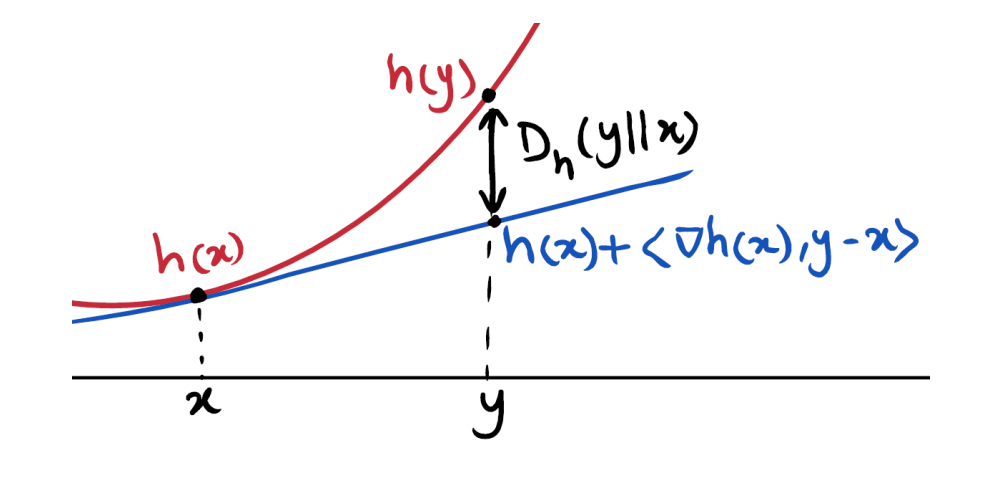
\includegraphics[width=0.5\textwidth]{figures/MD1.png}
    \caption{$D_h(y\|x)$ for the function $h:\RR \to \RR$}
\end{figure}
%────────────────────────────────────────


%────────────────────────────────────────
\begin{example}
[Examples of Bregman Divergence]
\label{eg: Examples of Bregman Divergence}
\begin{itemize}
    \item []
    \item For the function $h(x)=\frac{1}{2}\|x\|^2$, the Bregman divergence is
    $$
    D_h(y \| x)=\frac{1}{2}\|y\|^2-\frac{1}{2}\|x\|^2-\langle x, y-x\rangle=\frac{1}{2}\|y-x\|^2 .
    $$
    \item For the negative entropy function $h(x)=\sum_{i=1}^n\left(x_i \ln x_i-x_i\right)$, the Bregman divergence is
    $$
    D_h(y \| x)=\sum_{i=1}^n y_i \ln \frac{y_i}{x_i}-y_i+x_i .
    $$
    Assuming that $\sum_i y_i=\sum_i x_i=1$, we can simplify this to $\sum_i y_i \ln \frac{y_i}{x_i}$, which is the KL divergence.
\end{itemize}
\end{example}
%────────────────────────────────────────

Here are some properties of Bregman divergence. 

%────────────────────────────────────────
\begin{lemma}
[Three-point property]
\label{lem: Three-point property}
For $x, y, z \in \operatorname{dom}(h)$, we have
$$
D_h(x \| y)+D_h(z \| x)-D_h(z \| y)=\langle\nabla h(y)-\nabla h(x), z-x\rangle .
$$
\end{lemma}
%────────────────────────────────────────


%────────────────────────────────────────
\begin{lemma}
[Pythagoras theorem]
\label{lem: Pythagoras theorem}
Suppose that $C$ is a convex set, $x \in C$ and $y \in \mathbb{R}^d$. Then,
$$
D_h\left(x \| \Pi_C(y)\right)+D_h\left(\Pi_C(y) \| y\right) \leqslant D_h(x \| y),
$$
where
$$
\Pi_C^h(y)=\arg \min _{x \in C} D_h(x \| y) .
$$
\end{lemma}
%────────────────────────────────────────
%────────────────────────────────────────
\begin{proof}
    In terms of the definition of $\Pi_C(y)$, we have
    $$
    \left(\nabla h\left(\Pi_C(y)\right)-\nabla h(y) \right)^T\left(\Pi_C(y)-x\right) \leqslant 0,
    $$
    for any $x \in C$.
\end{proof}
%────────────────────────────────────────

\subsection{Changing the distance function}

We can replace $\frac{1}{2}\|x-y\|^2$ in \eqref{eq: non-cos PGD} with a generic Bregman divergence. Let's consider the unconstrained problem, then the update is:
$$
x_{t+1}=\arg \min _x\left\{\eta\left\langle\nabla f_t\left(x_t\right), x\right\rangle+D_h\left(x \| x_t\right)\right\} .
$$
Taking the derivative, we get
$$
\eta \nabla f_t\left(x_t\right)+\nabla h\left(x_{t+1}\right)-\nabla h\left(x_t\right)=0 .
$$
This gives us the update rule:
\begin{equation}
\label{eq: MD update rule}
    x_{t+1}=\nabla h^{-1}\left(\nabla h\left(x_t\right)-\eta \nabla f_t\left(x_t\right)\right) .
\end{equation}

\begin{algorithm}[H]
    \caption{Mirror Descent Algorithm}
    \label{MD algo}
    $x_1$ starting point \;
    \For{$t=1,2,\ldots,T$}{
        $x_{t+1}=\argmin_{x\in K} \{\eta \langle \nabla f_t(x_t), x \rangle + D_h(x\|x_t)\}$ \;
    }
\end{algorithm}
    
    %────────────────────────────────────────
    \begin{example}
    [Examples of mirror descent]
    \label{eg: Examples of mirror descent}
    \begin{itemize}
        \item []
        \item When $h(x)=\frac{1}{2}\|x\|^2$, the gradient $\nabla h(x)=x$, and the update rule becomes
        $$
        x_{t+1}=x_t-\eta \nabla f_t\left(x_t\right),
        $$
        the standard gradient descent update.
        \item When $h(x)=\sum_{i=1}^n\left(x_i \ln x_i-x_i\right)$, then $\nabla h(x)=\left(\ln x_1, \ldots, \ln x_n\right)$, and the update rule is
        $$
        \left(x_{t+1}\right)_i=\exp \left(\ln \left(x_t\right)_i-\eta \nabla f_t\left(x_t\right)_i\right)=\left(x_t\right)_i e^{-\eta \nabla f_t\left(x_t\right)_i} .
        $$
        
        This is exactly the update of the Hedge algorithm.
    \end{itemize}
    \end{example}
    %────────────────────────────────────────

    The same ideas also hold for constrained convex minimization: we now have to search for the minimizer with the set $K$. In this case, the algorithm using negative entropy resultsin the same Hedge-like update, following by scaling the point down to geta probability vector, thereby giving the probability values in Hedge.

    \begin{note}
        What would be the best choice of $h$ to minimize the function $f$ ? It would be $h=\eta f$, because adding $D_f\left(x \| x_t\right)$ to the linear approximation of $f$ at $x_t$ gives us back $f$. Of course, the update now requires us to minize $f(x)$, which is the origional problem. So we should coose an $h$ that is similar to $f$.
    \end{note}

    In summary, the algorithm tries to minimize the linear approximation of the function $f_t$ with respect to the Bregman divergence. Depending on the choice of the Bregman divergence, we can get different algorithms - this is the mirror descent framework.

\section{Mirror Descent: The Mirror Map View}
A different view of the mirror descent framework is the one originally presented by Nemirovsk and Yudin. They observe that in gradient descent, at each step we set $x_{t+1}=x_t-\eta f_t\left(x_t\right)$. However, \textbf{the gradient was actually defined as a linear functional on $\mathbb{R}^n$ and hence naturally belongs to the dual space of $\mathbb{R}^n$}. The fact that we represent this functional as a vecotr is a matter of convenience.

%────────────────────────────────────────
\begin{figure}[H]
    \centering
    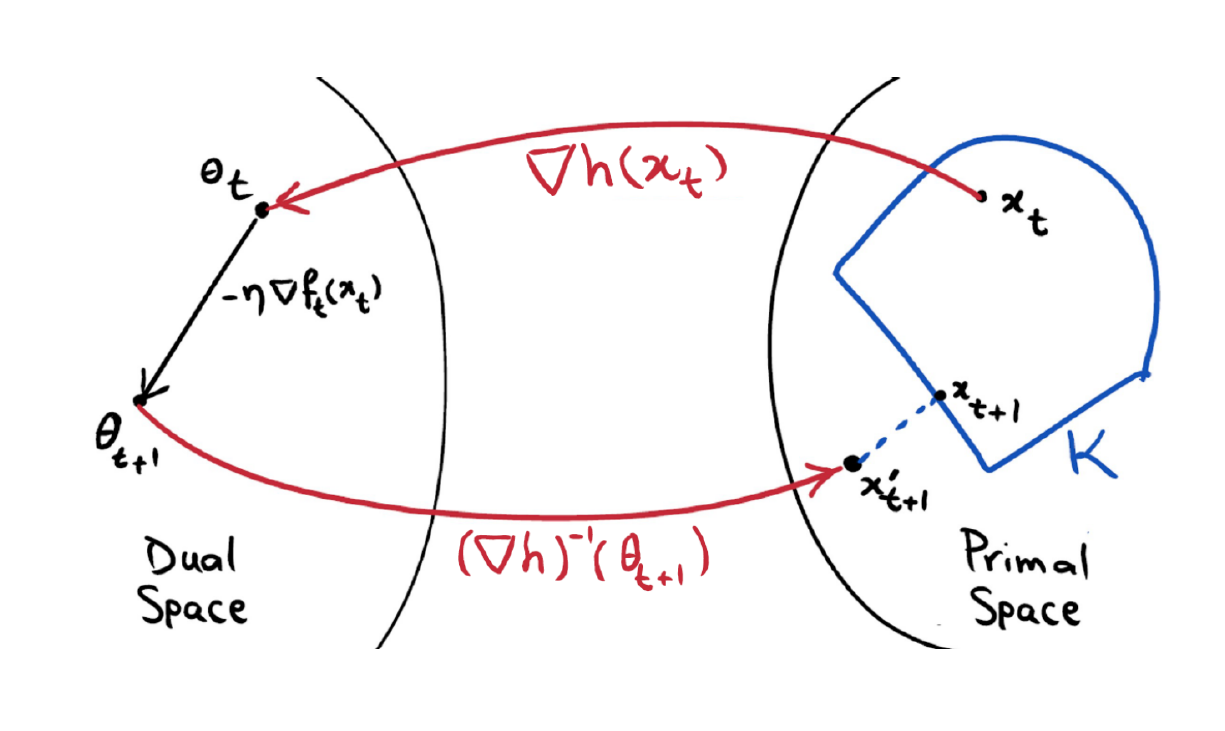
\includegraphics[width=0.5\textwidth]{figures/MD2.png}
    \caption{The mirror map view of mirror descent}
\end{figure}
%────────────────────────────────────────

In the vanilla graident descent method, we were working in $\mathbb{R}^n$ endowed with $\ell_2$-norm, and this normed space is self-dual. But when working with other normed spaces, adding a covector $\nabla f_t\left(x_t\right)$ to a vector $x_t$ might not be the right thing to do. Instead, Nemirovski and Yudin propose the following:

\begin{itemize}
    \item [1.] We map our current $x_t$ to a point $\theta_t$ in the dual space using a mirror map.
    \item [2.] Next we take the gradient step $\theta_{t+1}=\theta_t-\eta \nabla f_t\left(x_t\right)$.
    \item [3.] We map $\theta_{t+1}$ back to a point in the primal sapce $x_{t+1}^{\prime}$ using the inverse of the mirror map from Step 1 .
    \item [4.] If we are in the constrained case, this point $x_{t+1}^{\prime}$ might not be in the convex feasible region $K$, so we project it to a close point $x_{t+1}$ in $K$.
\end{itemize}

The name of the process comes from thinking of the dual space as being a mirror image of the primal space.

\subsection{Norms and their duals}
We skip the definition of norms. Now we consider a Hilbert space.

%────────────────────────────────────────
\begin{definition}
[Dual norm]
\label{def: Dual norm}
Given a linear space $C$ with norm $\|\cdot\|$, the dual norm $\|\cdot\|_*: C^* \rightarrow \mathbb{R}$ is defined as:
$$
\|y\|_*=\sup \{\langle x, y\rangle \mid\|x\| \leqslant 1, x \in C\} .
$$
\end{definition}
%────────────────────────────────────────


%────────────────────────────────────────
\begin{example}
[Exampls of dual norms]
\label{eg: Exampls of dual norms}
\begin{itemize}
    \item []
    \item Dual norm of $\ell_2$-norm is itself.
    \item Dual norm of Euclidean norm is itself.
    \item Dual norm of $\ell_p$-norm is $\ell_q$-norm, where $\frac{1}{p}+\frac{1}{q}=1$.
    \item Dual norm of $\ell_1$-norm is $\ell_{\infty}$-norm.
\end{itemize}
\end{example}
%────────────────────────────────────────


%────────────────────────────────────────
\begin{theorem}
[Cauchy-Schwarz for general norms]
\label{thm: Cauchy-Schwarz for general norms}
Given $x \in C, y\in C^*$, we have
$$
\langle x, y\rangle \leqslant\|x\|\|y\|_* .
$$
\end{theorem}
%────────────────────────────────────────


%────────────────────────────────────────
\begin{theorem}
[Self dual]
\label{thm: Self dual}
For a finite-dimensional space with norm $\|\cdot\|$, we have
$$
\left(\|\cdot\|_*\right)_*=\|\cdot\|.
$$
\end{theorem}
%────────────────────────────────────────

\subsection{Defining the mirror maps}
Now we define the mirror maps bsaed on a compact subspace $\cX$ of $\RR^n$.  



%────────────────────────────────────────
\begin{definition}
[Mirror map]
\label{def: Mirror map}
Let $\mathcal{D} \subset \mathbb{R}^n$ be a convex open set such that $\mathcal{X}$ is included in its closure, that is $\mathcal{X} \subset \overline{\mathcal{D}}$, and $\mathcal{X} \cap \mathcal{D} \neq \emptyset$. We say that $h: \mathcal{D} \rightarrow \mathbb{R}$ is a mirror map if it safisfies the following properties:
\begin{itemize}
    \item [1.] $h$ is strictly convex and differentiable.
    \item [2.] The gradient of $h$ takes all possible values, that is $\nabla h(\mathcal{D})=\mathbb{R}^n$.
    \item [3.] The gradient of $h$ diverges on the boundary of $\mathcal{D}$, that is
    $$
    \lim _{x \rightarrow \partial \mathcal{D}}\|\nabla h(x)\|=+\infty.
    $$
\end{itemize}
\end{definition}
%────────────────────────────────────────

In mirror descent the gradient of the mirror map $h$ is used to map points from the ``primal'' to the ``dual'' (note that all points lie in $\mathbb{R}^n$ so the notions of primal and dual spaces only have an intuitive meaning). Precisely a point $x \in \mathcal{X} \cap \mathcal{D}$ is mapped to $\nabla h(x)$, from which one takes a gradient step to get to $\nabla h(x)-\eta \nabla f(x)$. Property (ii) then allows us to write the resulting point as $\nabla h(y)=\nabla h(x)-\eta \nabla f(x)$ for some $y \in \mathcal{D}$. The primal point $y$ may lie outside of the set of constraints $\mathcal{X}$, in which case one has to project back onto $\mathcal{X}$. In mirror descent this projection is done via the Bregman divergence associated to $h$. 

%────────────────────────────────────────
\begin{example}
[Examples of mirror maps]
\label{eg: Examples of mirror maps}
\begin{itemize}
    \item []
    \item $h(x) = \frac{1}{2} \|x\|_2^2$ is $1$-strongly convex with respect to $\|\cdot \|_2$. 
    \item $h(x)= \sum_{i=1}^{n} x_i (\log x_i -1)$ is $1$-strongly convex with respect to $\|\cdot \|_1$.   
\end{itemize}
\end{example}
%────────────────────────────────────────

Then we just repeat the Nemirovski-Yudin process.

\section{Analysis}

Now we focus on the mirror descent with constrained convex minimization. Let $y_{t+1}\in \cD$ such that 
\begin{equation}
\label{eq: MD update yt}
    \nabla h(y_{t+1}) = \nabla h(x_t) - \eta \nabla f_t(x_t), 
\end{equation}
and 
\begin{equation}
\label{eq: MD update projection}
    x_{t+1} \in \Pi_{\cX}^{h}(y_{t+1}) = \argmin_{x\in \cX} D_h(x\|y_{t+1}).
\end{equation}

%────────────────────────────────────────
\begin{theorem}
[Online mirror descent regret bound]
\label{thm: Online mirror descent regret bound}
Let $\|\cdot\|$ be a norm on $\mathbb{R}^n$ and $h$ be an $\alpha$ strongly convex function with respect to $\|\cdot\|$. Given $f_1, \ldots, f_T$ be convex differentiable functions, the mirror descent algorithm starting with $x_1$ and taking constant step size $\eta$ in every iteraetion produces $x_1, \ldots, x_T$ such that for any $x^* \in \mathbb{R}^n$,
\begin{equation}
\label{eq: regret of MD}
    \sum_{t=1}^T f_t\left(x_t\right) \leqslant \sum_{t=1}^T f_t\left(x^*\right)+\underbrace{\frac{D_h\left(x^* \| x_1\right)}{\eta}+\frac{\eta \sum_{t=1}^T\left\|\nabla f_t\left(x_t\right)\right\|_*^2}{2 \alpha}}_{\text {regret }} .
\end{equation}
\end{theorem}
%────────────────────────────────────────
%────────────────────────────────────────
\begin{proof}
    For any $x\in \cX \cap \cD$, we have 
    \begin{align*}
        &f_t(x_t) - f(x) \\ 
        & \le \nabla f_t(x_t)^T(x_t  -x) &&\explain{ Convexity of $f$ } \\  
        & = \frac{1}{\eta }(\nabla h(x_t) - \nabla h(y_{t+1}))^\top (x_t - y_{t+1}) &&\explain{ By \eqref{eq: MD update yt} }  \\
        & = \frac{1}{\eta} \Big(D_h(x\|x_t) + D_h(x_t\|y_{t+1}) - D_h(x\|y_{t+1})\Big) &&\explain{ By \autoref{lem: Three-point property}} \\
        & \le \frac{1}{\eta} \Big (D_h(x\|x_t) + D_h(x_t\|y_{t+1}) - D_h(x\|x_{t+1}) - D_h(x_{t+1}\|y_{t+1})\Big) &&\explain{ By \autoref{lem: Pythagoras theorem}}. 
    \end{align*}
    The term $D_h(x\|x_t) -  D_h(x\|x_{t+1})$ will lead to a telescopic sum, and it remains to bound the other term as follows: 
    \begin{align*}
        &D_h(x_t\|y_{t+1}) - D_h(x_{t+1}\|y_{t+1}) \\ 
        &= h(x_{t} - h(x_{t+1}) - \nabla h(y_{t+1})^\top (x_t - x_{t+1}) \\ 
        &\le \left( \nabla h(x_t) - \nabla h(y_{t+1}) \right)^\top (x_t - x_{t+1}) - \frac{\alpha}{2} \|x_t - x_{t+1}\|^2 &&\explain{ By the strong convexity of $h$} \\ 
        & = \eta \nabla f_t(x_t) ^\top (x_t - x_{t+1}) - \frac{\alpha}{2} \|x_t - x_{t+1}\|^2 &&\explain{ By \eqref{eq: MD update yt}} \\
        & \le \eta \| \nabla f_t(x_t)\|_*\cdot \|x_t - x_{t+1}\| - \frac{\alpha}{2} \|x_t - x_{t+1}\|^2 &&\explain{ Cauchy-Schwarz} \\
        &\le \frac{\eta^2 \|\nabla f_t(x_t)\|_*^2}{2\alpha}. &&\explain{ By completing the square}
    \end{align*}
    Now we have proved that: 
    \[
        \sum_{t=1}^T\left(f_t(x_t)-f(x)\right) \leq \frac{D_{h}\left(x \| x_1\right)}{\eta}+\eta \frac{ \|\nabla f_t(x_t)\|_*^2 T}{2 \alpha}.
    \]
    This is equivalent to \eqref{eq: regret of MD}. 
    \end{proof}
    %────────────────────────────────────────

    %────────────────────────────────────────
\begin{theorem}
[Offline mirror descent regret bound]
\label{thm: Offline mirror descent regret bound}
Let $h$ be a mirror map which is $\alpha$-strongly convex on $\cX \cap D$ w.r.t. $\|\cdot \|$. Let $R^2 = \sup_{x\in \cX \cap \cD} D_h(x\|x_1)$, and $f$ be convex and $L$-Lipschitz w.r.t. $\|\cdot \|$. Then the mirror descent with $\eta = \frac{R}{L}\sqrt{\frac{2\alpha}{T}}$ satisfies 
\[
    f\left(\frac{1}{T} \sum_{t=1}^T x_t\right)-f\left(x^*\right) \leq R L \sqrt{\frac{2}{\alpha T}}. 
\] 
\end{theorem}
%────────────────────────────────────────
%────────────────────────────────────────
\begin{proof}[Proof sketch]
Apply \autoref{thm: Online mirror descent regret bound} with $ \eta = \frac{R}{L}\sqrt{\frac{2\alpha}{T}}$. 
\end{proof}
%────────────────────────────────────────

\begin{note}
The MD convergence rate $O(1 / \sqrt{t})$ is slow. However, this is the best possible rate one can expect when solving nonsmooth large-scale convex problems represented by FO oracles, or any other oracles providing local information.
\end{note}

In fact, we have the following bad news. 

%────────────────────────────────────────
\begin{example}
[Lower bound example]
\label{eg: Lower bound example}
Consider convex minimization problem 
\begin{equation}
\label{eq: Lower bound example}
\tag{P}
        x_* = \argmin_{\|x\|\le R} f(x),
\end{equation}

where $\|\cdot \|$ is either the norm $\|\cdot \|_p$ on $\RR^n$ or the nuclear norm on $\RR^{n\times n}$. Let $f_* = \min _{\|x\|\le R} f(x)$ and 
\[
    \cF(L) = \{f: \RR^n \to \RR \mid f \text{ is $L$-Lipschitz w.r.t. $\|\cdot \|$}\}, 
\]
and asumme that when solving \eqref{eq: Lower bound example}, we have access to an first order oracle. Then for any $t\le n$ and $t$-step algorithm $\cB$ that solves \eqref{eq: Lower bound example} with an FO oracle, we have 
\[
    \sup_{f\in \cF(L)} \Big [ (f x_\beta(f)) - f_* \Big]  \ge 0.01 \frac{LR}{\sqrt{t} }.  
\]
Here $x_\beta(f)$ is the output of $\cB$ on the function $f$.
\end{example}
%────────────────────────────────────────
